\documentclass[xcolor=table]{beamer}
\usepackage{beamerthemesplit}
\usepackage{wrapfig}
\usetheme{SPbGU}
\usepackage{pdfpages}
\usepackage{amsmath}
\usepackage{cmap}
\usepackage[T2A]{fontenc}
\usepackage[utf8]{inputenc}
\usepackage[english,russian]{babel}
\usepackage{indentfirst}
\usepackage{amsmath}
\usepackage{tikz}
\usepackage{multirow}
\usepackage[noend]{algpseudocode}
\usepackage{algorithm}
\usepackage{algorithmicx}
\usepackage{fancyvrb}
\usetikzlibrary{shapes,arrows}
%usepackage{fancyvrb}
%\usepackage{minted}
%\usepackage{verbments}
\usepackage{fontawesome}

\beamertemplatenavigationsymbolsempty

\title[TM $\to$ G]{Реализация алгоритма построения представления группы по машине Тьюринга}
\institute[СПбГУ]{
JetBrains Research, Programming Languages and Tools Lab  \\
Санкт-Петербургский государственный университет \\
Системное программирование
}

\author[Шамрай Максим]{
\textbf{Автор:} Шамрай Максим Борисович \\
{\footnotesize
\textbf{Научный руководитель:} доцент, к.~ф.-м.н. Григорьев С. В.
\newline
\textbf{Рецензент:} ведущий инженер ООО "Ланит-Терком" Смирнов К. К.}}

\date{21.05.2020}

\begin{document}
{
\begin{frame}[fragile]
  \begin{tabular}{p{2cm} p{7.5cm} p{1cm}}
   \begin{center}
      
\includegraphics[height=1.5cm]{pictures/jetbrainsResearch.pdf}
    \end{center}
    &
    \begin{center}
      
\includegraphics[height=1.5cm]{pictures/SPbGU_Logo.png}
    \end{center}
    &
    \begin{center}
      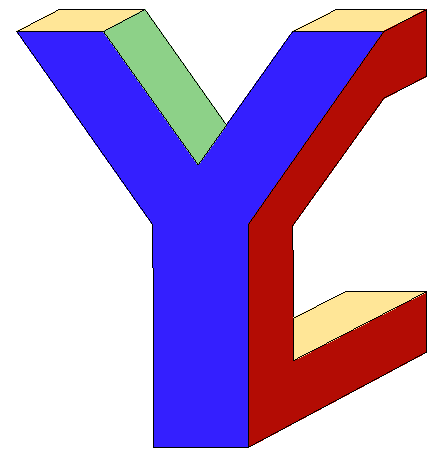
\includegraphics[height=1.5cm]{pictures/YC_logo.pdf}
    \end{center}
  \end{tabular}
  \titlepage
\end{frame}
}


\begin{frame}[fragile]
 \frametitle{Мотивация}
\begin{itemize}
    \item Кроме иерархии Хомского, есть довольно много классов формальных языков, например, конъюнктивные и Булевы
    \item Не у всех есть критерий непредставимости языка в классе ($Conj \subseteq Bool$ ?)
    \item В последнее время все чаще прибегают к смежным дисциплинам для исследования языков
    \item Предлагается построить представление группы по языку, чтобы в дальнейшем можно было применять аппарат теории групп для исследований
\end{itemize}
\end{frame}

\begin{frame}[fragile]
 \frametitle{Представление группы}
        Пусть $\Sigma$ --- конечный алфавит,
        
        $\Sigma^{-1} = \{ a^{-1}~|~a \in \Sigma, \, 
        a a^{-1} = a^{-1} a = 1_G \}$, тогда
    \begin{itemize}
        \item $\Sigma^+$ --- свободная полугруппа
        \item $\Sigma^*$ --- свободный моноид
        \item $(\Sigma \cup \Sigma^{-1})^*$ --- свободная группа
    \end{itemize}
    
    \pause
        $G = \langle A~|~R \rangle$ --- представление группы
    \begin{itemize}
        \item $G = \langle a, b~|~a^3, b^2, (ab)^2 \rangle = \{\varepsilon, a, a^2, b, ab, a^2b\} = S_3$
        \item $G = \langle a~|~a^5\rangle = Z_5$
        \item $G = \langle a, b~|~aba^{-1}b^{-1} \rangle$
    \end{itemize}
\end{frame}

\begin{frame}[fragile]
 \frametitle{Связь формальных языков с теорией групп}
    \begin{itemize}
        \item Представления групп описывают языки, которые могут быть заданы следующим выражением: $L(G) = \{\omega = 1_G ~|~ \omega \in (A \cup A^{-1})^*\}$
        \item Построение представления группы по машине Тьюринга, которая распознает некоторый язык, было описано в статье\footnote{Mark V. Sapir, Jean-Camille Birget and Eliyahu Rips "Isoperimetric and Isodiametric Functions of Groups" (2002)}
    \end{itemize}
    \begin{block}{Теорема 1}
		Пусть $L \subseteq \Sigma^+$ язык, принимаемый машиной Тьюринга $M$,
    тогда существует конечно представленная группа $G(M)=\langle A~|~R \rangle$
    и инъективное отображение $K: \Sigma^+ \to (A \cup A^{-1})^+$ такое что:
    $u \in L \iff K(u)=1_G$
	\end{block}
\end{frame}

\begin{frame}[fragile]{Постановка задачи}
\textbf{Цель:} Предоставить исследователям возможность ставить вычислительные эксперименты по преобразованию формального языка в соответствующее представление группы
\newline
\newline
\textbf{Задачи:}
    \begin{enumerate}
    \item Реализовать алгоритм преобразования контекстно-свободной грамматики в машину Тьюринга
    \item Реализовать алгоритм построения представления группы по машине Тьюринга
    \item Разработать интерпретаторы промежуточных машин для проверки сохранения языка
    \item Провести эксперименты
\end{enumerate}
\end{frame}

\begin{frame}[fragile]{Схема построения представления группы}
\begin{figure}[H]
  \centering
  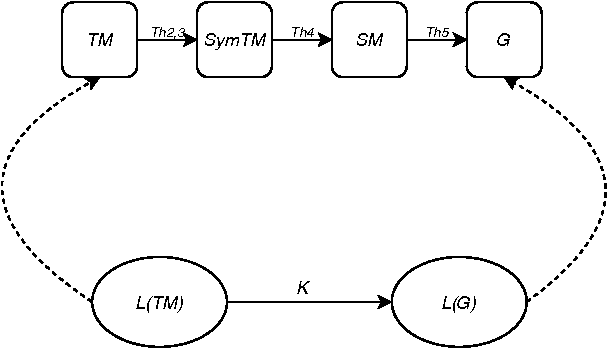
\includegraphics[width=120mm]{pictures/2.pdf}
 \end{figure}
\end{frame}

\begin{frame}[fragile]{Нотация машины Тьюринга}
Машина Тьюринга имеет $ k $ лент и $ k $ голов и может быть описана как шестиместный кортеж:
$M = \langle X, \Gamma, Q, \Theta, \overline{s_1}, \overline{s_0} \rangle$,
где
\begin{itemize}
    \item $X$ --- входной алфавит.
    \item $\Gamma$ --- алфавит лент.
    \item $Q = \cup_{i=1}^k Q_i$ --- множество состояний голов на лентах машины.
    \item $\Theta$ --- множество команд машины.
    \item $\overline{s_1}$ --- k-вектор начальных состояний машины.
    \item $\overline{s_0}$ --- k-вектор конечных состояний машины.
\end{itemize}

Команда одноленточной машины Тьюринга имеет вид: 
\begin{center}
    $u q v \to u' q' v'$
\end{center}
где $u, v, u', v'$ --- ячейки, $q, q'$ --- состояния

\end{frame}

\begin{frame}[fragile]{Построение распознавателя контекстно-свободной грамматики}
    \begin{itemize}
        \item Алгоритм строит магазинный автомат, написанный в терминах машины Тьюринга, по контекстно-свободной грамматике
        \begin{itemize}
            \item На входе --- контекстно-свободная грамматика в нормальной форме Хомского
            \item На выходе --- машина Тьюринга, где первая лента входная, а вторая эмулирует стек автомата
        \end{itemize}
        \item Для построения детерминированной машины Тьюринга по детерминированной грамматике при необходимости добавляются команды предпросмотра
    \end{itemize}
\end{frame}

\begin{frame}[fragile]{Симметризация недетерминированной машины Тьюринга}
\begin{block}{Теорема 2}
Для любой машины Тьюринга M существует недетерминированная машина Тьюринга M' со следующими свойствами:
    \begin{itemize}
        \item M' симметричная
        \item Распознает тот же язык, что и M
        \item Каждая команда действует только на одной ленте
    \end{itemize}
\end{block}
\begin{itemize}
    \item Для сохранения языка добавляется лента, алфавитом которой яляются команды машины Тьюринга
    \item Получившаяся симметричная машина Тьюринга может иметь много состояний и состоять из многих команд, что говорит о ее сложности 
    \item Но при этом ее можно построить и для детерминированной, и для недетерминированной исходной машины Тьюринга
\end{itemize}
\end{frame}

\begin{frame}[fragile]{Симметризация детерминированной машины Тьюринга}
    \begin{block}{Теорема 3}
    Для любой детерминированной машины Тьюринга M существует эквивалентная симметричная машина Тьюринга, полученная из M добавлениями команд $\tau^{-1}$ для каждой команды $\tau$ из M.
	\end{block}
	\begin{itemize}
	    \item Авторы теоремы E. Post и A. A. Markov (1947)
	    \item Получившаяся симметричная машина Тьюринга гораздо легче машины, полученной по предыдущей теореме
	    \item Но ее можно построить только для детерминированной машины Тьюринга
	\end{itemize}
\end{frame}

\begin{frame}[fragile]{Построение представления группы}

S-машина --- система переписывания символов на ленте, которая поддерживает обратный алфавит.

\begin{block}{Теорема 4}
Для любой машины Тьюринга M' существует S-машина, которая симулирует M'
\end{block}

\begin{block}{Теорема 5}
Для любой S-машины существует соответствующая конечно-представленная группа
\end{block}
\end{frame}

\begin{frame}[fragile]{Архитектура решения\footnote{\url{https://github.com/YaccConstructor/LangToGroup}}}
\begin{figure}[H]
  \centering
  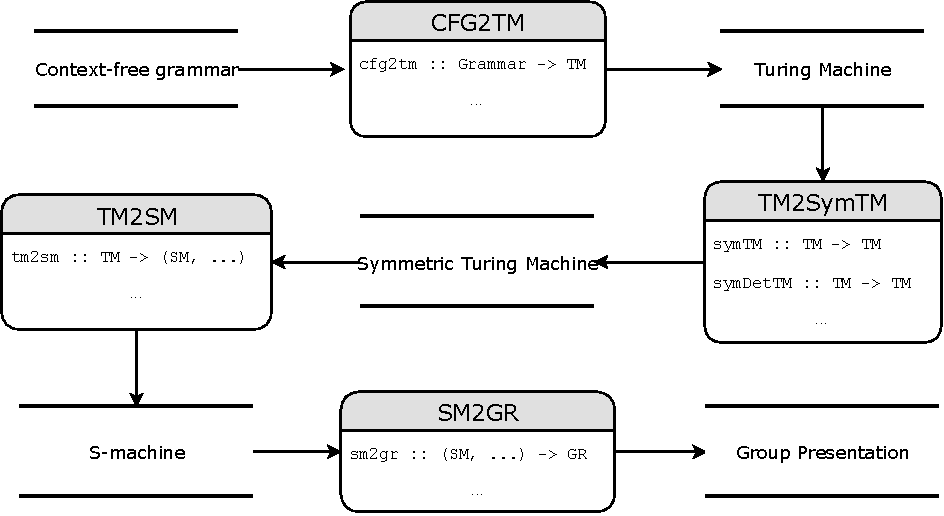
\includegraphics[width=120mm]{pictures/diplomaSmallUML.pdf}
 \end{figure}
\end{frame}

\begin{frame}[fragile]{Интерпретация}
\begin{itemize}
    \item Необходимо проверять, сохраняется ли язык после каждого шага преобразования
    \item Так как авторы статьи используют свою эквивалентную нотацию машины Тьюринга, нами были разработаны интерпретаторы и S-машины, и машины Тьюринга 
    \begin{itemize}
        \item Дерево вычислений, корень --- стартовая конфигурация
        \item Обход дерева в ширину
        \item В интерпретаторе S-машины используется множество пройденных конфигураций и построение дерева определенной высоты с выводом в DOT (graph description language)
    \end{itemize}
\end{itemize}
\end{frame}

\begin{frame}[fragile]{Эксперименты}
Для оценки размера получившегося представления группы, запустили алгоритмы с недетерминированной и детерминированной симметризацией на трех грамматиках:
\begin{columns}[onlytextwidth,T]
        \column{\dimexpr\linewidth/2}
        \begin{itemize}
    \item one rule: 
    $\begin{array}{lCr}
        \nonumber S \to a
    \end{array}$
    \newline
    \newline
    \item $a^*$:
    $\begin{array}{lCr}
        S \to AS ~|~ \varepsilon \nonumber \\
        A \to a \nonumber
    \end{array}$
    \end{itemize}
    
        \column{\dimexpr\linewidth/2}
        \begin{itemize}
            \item Dyck:
    $\begin{array}{lCr}
        S \to AC ~|~ \varepsilon \nonumber \\
        C \to SD \\
        D \to BS \nonumber \\
        A \to a \nonumber \\
        B \to b \nonumber
    \end{array}$
        \end{itemize}
    \end{columns}

\end{frame}

\begin{frame}[fragile]{Эксперименты\footnote{Используя алгоритм симметризации недетерминированных машин Тьюринга}}

В таблице приведены мощности множеств

\begin{table*}
\begin{center}
\begin{tabular}{|c!{\vrule width 1pt}
c|c|c!{\vrule width 1pt}
c|c|c|c|}
\hline
&
\multicolumn{3}{|c|}{\textbf{Grammar}}&
\multicolumn{4}{|c|}{\textbf{TM}}\\
\cline{2-8}
&$\Sigma$&$N$&$R$
&$X$&$\Gamma$&$Q$&$\Theta$\\
\hline
1 rule
&1&1&1
&1&3&6&5\\
\hline
$a^*$
&1&2&3
&1&4&8&10\\
\hline
Dyck
&2&4&6
&2&8&13&21\\
\hline
\end{tabular}
\end{center}
\end{table*}


\begin{table*}
\begin{center}
\begin{tabular}{
|c|c|c|c!{\vrule width 1pt}
c|c|c!{\vrule width 1pt}
c|c|}
\hline
\multicolumn{4}{|c|}{\textbf{TM'}}&
\multicolumn{3}{|c|}{\textbf{SM}}&
\multicolumn{2}{|c|}{\textbf{G}}\\
\cline{1-9}
$X$&$\Gamma$&$Q$&$\Theta$
&$Y$&$Q$&$\Theta$
&$A$&$R$\\
\hline
1&14&270&206
&14&88246&2363
&89508&56187\\
\hline
1&26&547&434
&26&344118&5741
&347370&204903\\
\hline
2&54&1131&900
&54&1469136&15064
&1478859&957619\\
\hline
\end{tabular}
\end{center}
\end{table*}
\end{frame}

\begin{frame}[fragile]{Эксперименты\footnote{Используя алгоритм симметризации детерминированных машин Тьюринга}}

В таблице приведены мощности множеств

\begin{table*}
\begin{center}
\begin{tabular}{|c!{\vrule width 1pt}
c|c|c!{\vrule width 1pt}
c|c|c|c|}
\hline
&
\multicolumn{3}{|c|}{\textbf{Grammar}}&
\multicolumn{4}{|c|}{\textbf{TM}}\\
\cline{2-8}
&$\Sigma$&$N$&$R$
&$X$&$\Gamma$&$Q$&$\Theta$\\
\hline
1 rule
&1&1&1
&1&3&6&5\\
\hline
$a^*$
&1&2&3
&1&4&8&10\\
\hline
Dyck
&2&4&6
&2&8&13&21\\
\hline
\end{tabular}
\end{center}
\end{table*}


\begin{table*}
\begin{center}
\begin{tabular}{
|c|c|c|c!{\vrule width 1pt}
c|c|c!{\vrule width 1pt}
c|c|}
\hline
\multicolumn{4}{|c|}{\textbf{TM'}}&
\multicolumn{3}{|c|}{\textbf{SM}}&
\multicolumn{2}{|c|}{\textbf{G}}\\
\cline{1-9}
$X$&$\Gamma$&$Q$&$\Theta$
&$Y$&$Q$&$\Theta$
&$A$&$R$\\
\hline
1&6&39&34
&6&6058&501
&6410&7637\\
\hline
1&8&73&72
&8&15888&1024
&16565&17657\\
\hline
2&16&161&158
&16&67754&2837
&69772&71533\\
\hline
\end{tabular}
\end{center}
\end{table*}
\end{frame}

\begin{frame}[fragile]{Эксперименты}
    \begin{itemize}
    \item Размер получившихся представлений групп при симметризации в детерминированном случае гораздно меньше
    \begin{itemize}
        \item Чем меньше получившееся предсталение группы, тем проще потом сказать о словах в группе, которые равны единице
        \item В случае детерминированных грамматик, нужно использовать симметризацию для детерминированных машин
    \end{itemize}
    \item Проведены эксперименты по интерпретации слов представлений групп
    \begin{itemize}
        \item Математические пакеты Gap и Maple не справились с задачей проверки слов на равенство групповой единице
        \item Актуальным остается вопрос разработки эффективного алгоритма интерпретации слов представлений групп
    \end{itemize}
    \end{itemize}
\end{frame}

\begin{frame}[fragile]{Результаты}
    \begin{enumerate}
    \item Реализован алгоритм преобразования контекстно-свободной грамматики в машину Тьюринга
    \item Реализован алгоритм построения представления группы по машине Тьюринга
    \item Разработаны интерпретаторы промежуточных машин для проверки сохранения языка в ходе преобразований
    \item Проведен ряд экспериментов
\end{enumerate}
\end{frame}

\begin{frame}[noframenumbering]{Проблема слов}
    \begin{columns}[onlytextwidth,T]
        \column{\dimexpr\linewidth-60mm-5mm}
        $G = \langle A~|~R \rangle$, $\Sigma = A \cup A^{-1}$
        
        $\phi : \Sigma^* \to G$
        
        $W(G) = \phi^{-1}(1)$
        \newline
        \newline
        \begin{itemize}
            \item $W(G)$ -- регулярна $\iff G$ -- конечна (Anisimov)
            \item $W(G)$ -- контекстно-свободна $\iff \exists H < G$ -- конечного идекса (Muller–Schupp)
        \end{itemize}
        
        \column{60mm}
        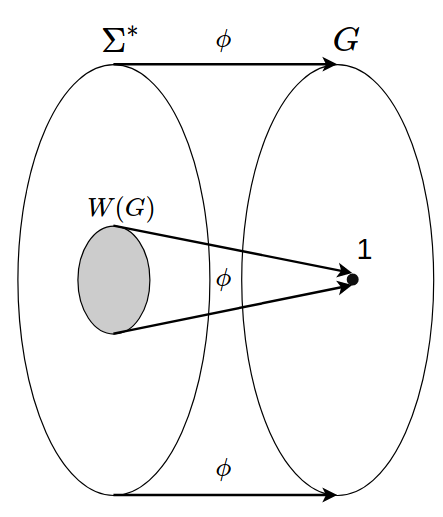
\includegraphics[width=60mm]{pictures/3.png}
    \end{columns}
\end{frame}

\end{document}
